
\usecaseristoratore{Modifica menù}
\label{usecase:Modifica menù}


\begin{figure}[h]
	\centering
	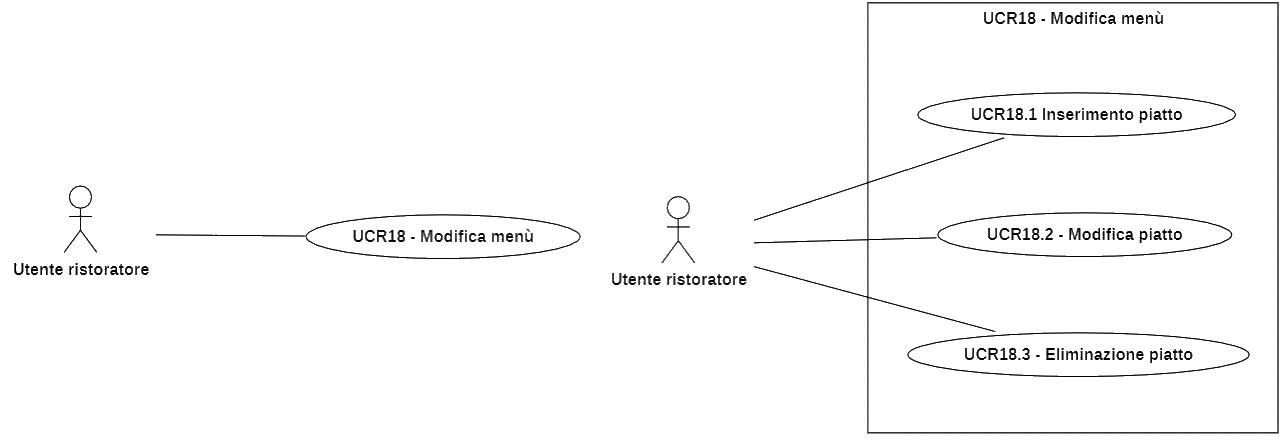
\includegraphics[width=0.99\textwidth]{./uml/UCR18.png} 
	\caption{Modifica menù}
	\label{fig:UCR18}
  \end{figure}

\begin{itemize}
	\item \textbf{Attore principale:} Utente ristoratore.

	\item \textbf{Precondizione:} L'Utente ristoratore ha effettuato l'accesso al Sistema (vedi \autoref{usecase:Effettua accesso}).

	\item \textbf{Postcondizione:} L'Utente ristoratore gestisce il menù del proprio ristorante.


	\item \textbf{Scenario principale:}
	      \begin{enumerate}

		      \item L'Utente ristoratore può compiere le seguenti azioni per quanto riguarda la gestione del menù:
		      \begin{itemize}
                \item Inserimento di un piatto nel menù (vedi \autoref{usecase:Inserimento piatto}).
                \item Modifica di un piatto nel menù (vedi \autoref{usecase:Modifica piatto}).
                \item Eliminazione di un piatto nel menù (vedi \autoref{usecase:Eliminazione piatto}).
              \end{itemize}
		      \item Il Sistema registra le modifiche apporate al menù da parte del ristoratore.

	      \end{enumerate}
\end{itemize}

\subusecaseristoratore{Inserimento piatto}
\label{usecase:Inserimento piatto}
\begin{itemize}

	\item \textbf{Attore principale:} Utente ristoratore.

	\item \textbf{Precondizione:} L'Utente ristoratore si trova nella sezione di gestione del menù (vedi \autoref{usecase:Modifica menù}).

	\item \textbf{Postcondizione:} L'Utente ristoratore ha inserito un piatto nel menù.

	\item \textbf{Scenario principale:}
	\begin{enumerate}
		\item L'Utente ristoratore inserisce un nuovo piatto nel menù;
		\item Il Sistema aggiorna il menù con il nuovo piatto inserito dal ristoratore.
	\end{enumerate}

\end{itemize}


\subusecaseristoratore{Modifica piatto}
\label{usecase:Modifica piatto}
\begin{itemize}

	\item \textbf{Attore principale:} Utente ristoratore.

	\item \textbf{Precondizione:} L'Utente ristoratore si trova nella sezione di gestione del menù (vedi \autoref{usecase:Modifica menù}).

	\item \textbf{Postcondizione:} L'Utente ristoratore ha modificato un piatto nel menù.

	\item \textbf{Scenario principale:}
	\begin{enumerate}
		\item L'Utente ristoratore modifica un piatto nel menù;
		\item Il Sistema aggiorna il menù con il piatto modificato dal ristoratore.
	\end{enumerate}

\end{itemize}


\subusecaseristoratore{Eliminazione piatto}
\label{usecase:Eliminazione piatto}
\begin{itemize}

	\item \textbf{Attore principale:} Utente ristoratore.

	\item \textbf{Precondizione:} L'Utente ristoratore si trova nella sezione di gestione del menù (vedi \autoref{usecase:Modifica menù}).

	\item \textbf{Postcondizione:} L'Utente ristoratore ha eliminato un piatto nel menù.

	\item \textbf{Scenario principale:}
	\begin{enumerate}
		\item L'Utente ristoratore eliminato un nuovo piatto nel menù;
		\item Il Sistema aggiorna il menù con il piatto eliminato dal ristoratore.
	\end{enumerate}

\end{itemize}
